% !TEX root = ../../main.tex
% !TEX spellcheck = en_US
We begin by describing the main features, behaviors, and goals of our bot; these features have been selected by either what players wanted, 0what we think would be a good feature, or both and then testing what works and what does not. We then give a brief overview of the system and how the different components/classes work and communicate with each other to get a quick grasp how everything is connected.

After the overview we will give a detailed description of all the important features of the classes, giving motivations of our design choices. The design choices were selected by either research, common knowledge in the StarCraft community, what we think would be good, or a mix of any and then testing what works and what does not, first on ourselves and then, close to the end, on our test players to find weird and non-acceptable behaviors.

\paragraph{Configurable variables}
Many fixed variables in BATS are configurable from a config.ini file. This design choice was made to easily tweak these variables in-game, instead of having to recompile, start the game, wait until the game state is present (necessary buildings have been built). The configuration file could be reloaded anytime in-game using \emph{/reload config} command. Throughout the method section these will be presented with their current value, variables that are configurable will have a superscript of \conf attached to it, e.g. 150\conf seconds. If a range has a superscript, e.g. [0.0, 1.0]\conf both 0.0 and 1.0 is configurable.

\paragraph{Terminology explained}
There are a couple of words that needs to be explained before digging into the details.

\begin{description}
	\item[Region \& choke point] A typical map from StarCraft contains many regions, the regions are (often) big open spaces divided by choke points—narrow paths, e.g. paths moving up or down a cliff. A region could be fully isolated, this means it can only be reached by air—BATS does not work on these kind of maps, all regions must be connected in one way or the other. Regions and choke points are illustrated in figure \ref{fig:region_and_choke_points}—this is also the map we used for all our tests.
	\item[Squad] Units grouped together with a common goal or behavior, such as attack squad or scout squad.
	\item[Allied/enemy squad] A virtual squad used to group close allied or enemy units together.
	\item[Expanding] The time when from one want to build another base (to mine minerals and gas from) until the base has completed.
\end{description}
\begin{figure}[htb]
	\centering
	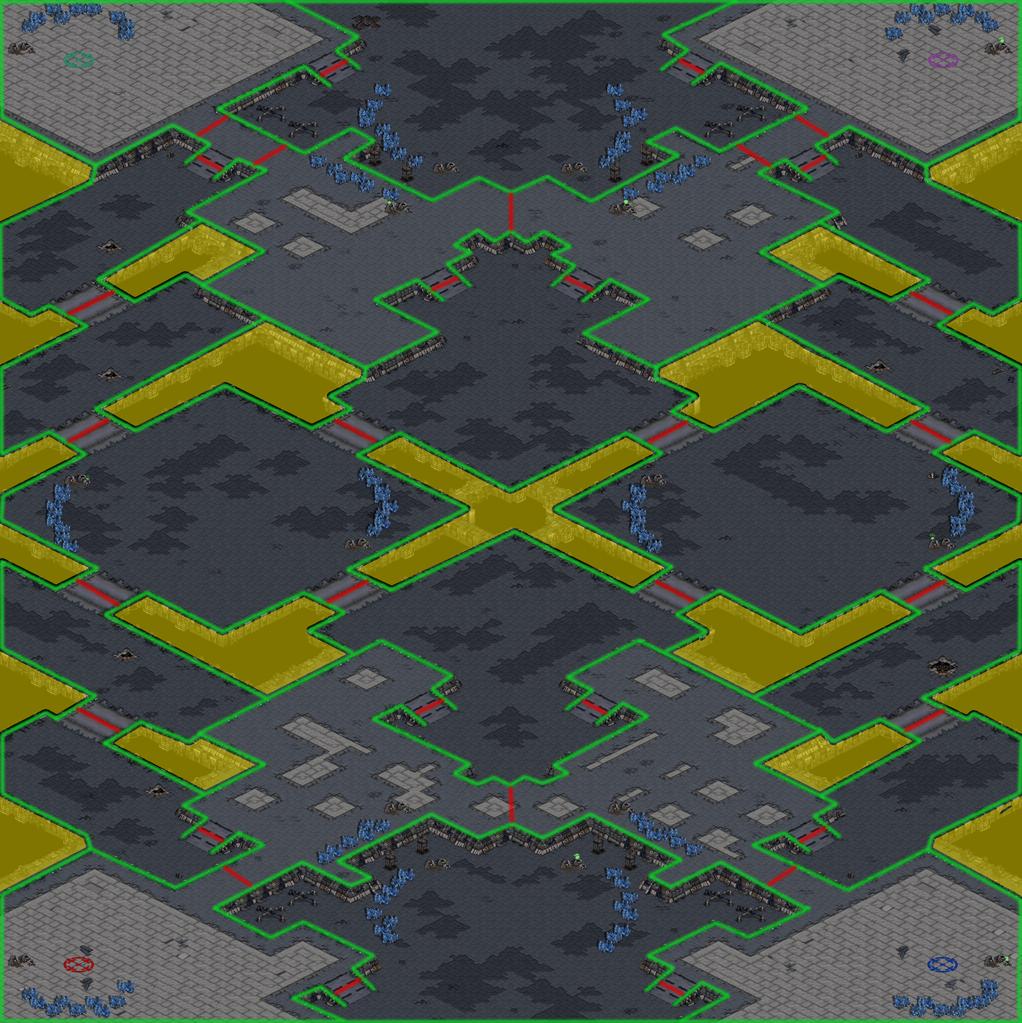
\includegraphics[width=0.8\textwidth]{space_atoll_(co-op)_regions_small}
	\caption[Regions and choke points]{Regions and choke points. Regions are surrounded by green lines, choke points are denoted by a red line, and the yellow areas are unwalkable terrain.}
	\label{fig:region_and_choke_points}
\end{figure}